\documentclass[12pt]{article}
\usepackage{amsmath,amsfonts,times}
\usepackage{graphicx,color,tikz,pgfplots}
\usepackage[zswash]{mtpro2}
\usepackage[paperwidth=8.1cm,paperheight=8.1cm,lmargin=0in,rmargin=0in,tmargin=0.in,bmargin=0.in]{geometry}
\usepackage{bm}
\usetikzlibrary{arrows,shadings,shapes.arrows,decorations.pathreplacing,calc, positioning}
\usepgfplotslibrary{fillbetween}

\begin{document}
\centering
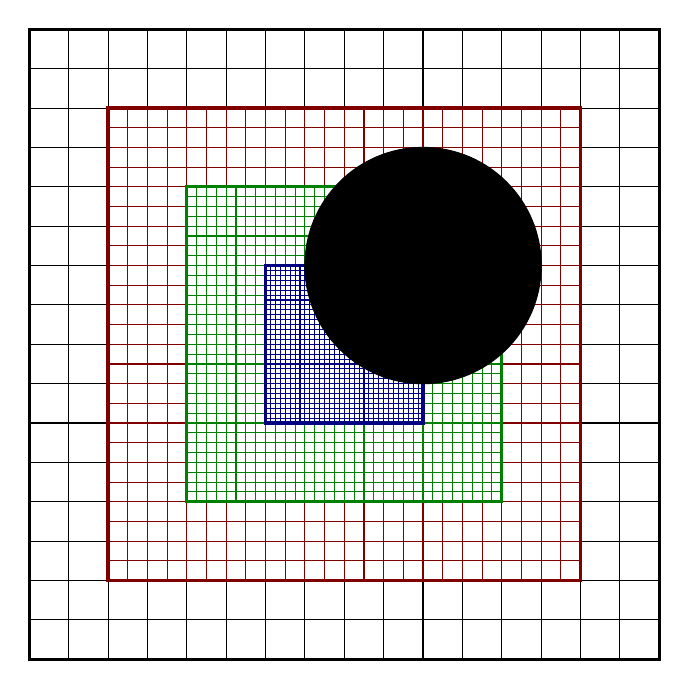
\begin{tikzpicture}[on grid]
  \fill[white,fill opacity=1] (0,0) rectangle (8,8);
  \draw[step=5mm, black, thin] (0,0) grid (8,8); %defining grids
  \draw[black,very thick] (0,0) rectangle (8,8);%marking borders

  \fill[white,fill opacity=1] (1,1) rectangle (7,7);
  \draw[step=2.5mm, red!50!black, thin] (1,1) grid (7,7);  %Nested grid 1
  \draw[red!50!black, very thick] (1,1) rectangle (7,7);%marking borders

  \fill[white,fill opacity=1] (2,2) rectangle (6,6);
  \draw[step=1.25mm, green!50!black,thin] (2,2) grid (6,6);  %Nested grid 2
  \draw[green!50!black, very thick] (2,2) rectangle (6,6);%marking borders

  \fill[white,fill opacity=1] (3,3) rectangle (5,5);
  \draw[step=0.625mm, blue!50!black,thin] (3,3) grid (5,5);  %Nested grid 3
  \draw[blue!50!black, very thick] (3,3) rectangle (5, 5);

  \draw[black, fill=black] (5,5) circle (1.5cm);
\end{tikzpicture}

\end{document} 
